\documentclass[aspectratio=169]{beamer}	% TPU recommends 16:9 ratio, 4:3 may require some work with inner theme .sty file

% Style options:
% light --- light theme (default)
% dark --- dark theme
% enlogo --- english TPU logo {default}
% rulogo --- russian TPU logo

\usetheme[dark]{tpu}		% dark theme used as an example of optional argument

%\usepackage[russian]{babel}		%uncomment this to work in russian
\usepackage[utf8]{inputenc}
\usepackage[T2A]{fontenc}

\usepackage{booktabs}	% good looking tables
\usepackage{multicol}	% text in multiple columns, useful for side-by-side text and pictures

\hyphenpenalty=10000	% i don’t think hyphenation in presentations is a good idea, feel free to change however you like

\title{Example TPU presentation}
\subtitle{Made possible by \LaTeX\ and Beamer}
\author{Author can be on \\ several lines}
\date{\today}

\begin{document}

% notice usage of \titleframe and several other unconventional functions
% the reason being is custom backgrounds on these slides

\titleframe		% title

\tocframe{}		% this custom frame accepts options for ToC

\section{Colours}

\sectionframe	% section title is automatically capitalised

\begin{frame}[fragile]
\frametitle{Bullets and alerted text}
Environment \verb"itemize" has green bullets:
\begin{itemize}
	\item first item
	\item second item
	\item third item
\end{itemize}

Also notice that \alert{alerted} text is green. Bullets and alerted text are {\color{tpugreen}light green} on dark background and {\color{tpudarkgreen}dark green} --- on light
\end{frame}

\begin{frame}[fragile]
\frametitle{More colours}
There are also several pre-defined colours for usage in tables and graphs
\begin{table}
\begin{center}
\begin{tabular}{ *{2}{c l} }
	\begin{tikzpicture}\fill[color = extragreen] (0,0) rectangle (1,0.5);\end{tikzpicture} & \verb"extragreen" & \begin{tikzpicture}\fill[color = extrared] (0,0) rectangle (1,0.5);\end{tikzpicture} & \verb"extrared" \\
	\begin{tikzpicture}\fill[color = extrablue] (0,0) rectangle (1,0.5);\end{tikzpicture} & \verb"extrablue" & \begin{tikzpicture}\fill[color = extraorange] (0,0) rectangle (1,0.5);\end{tikzpicture} & \verb"extraorange"
\end{tabular}
\end{center}
\end{table}%
\end{frame}

\section{Graphics}

\sectionframe

\subsection{Pictures}

\begin{frame}[fragile]
\frametitle{Pictures}
\begin{multicols}{2}
Pictures can be placed like in every \LaTeX\ document

Package \verb"multicol" is useful for side-by-side composition

There are several pictures provided by TPU as backgrounds for slides, look at \verb"beamerinnerthemetpu.sty" to learn~more
\columnbreak
\begin{figure}
\begin{center}
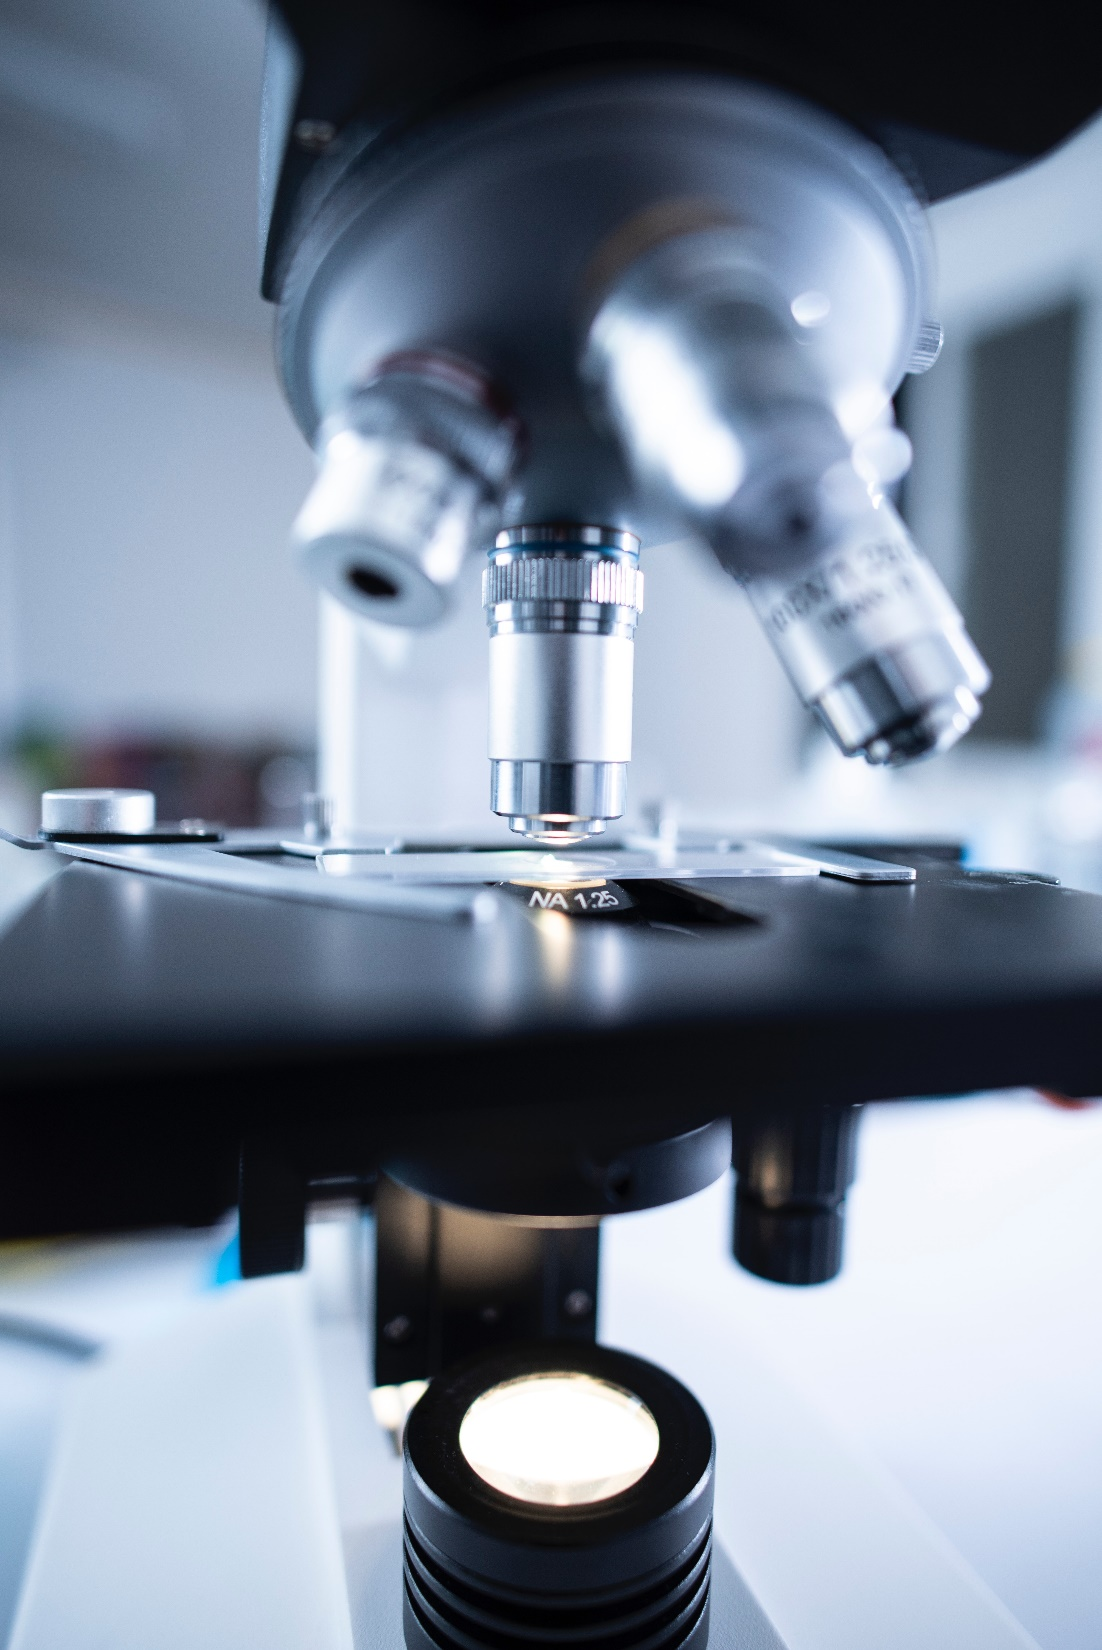
\includegraphics[height=0.6\textheight]{bgs/titlemicroscope}
\end{center}
\end{figure}
\end{multicols}
\end{frame}

\subsection{Icons}

\frame{
\frametitle{Icons}
TPU provides icons for most popular social networks. These can be seen used on the `Contacts' frame. Example of usage:


\includegraphics[height=0.6\baselineskip]{icons/white/twitter} @tpu	% icon can be placed more beautiful using TikZ, but this is just an example

Icons not related to social networks can be found on the TPU website
}

\section{Extras}

\sectionframe

\frame{
	\frametitle{Citation}
\begin{tikzpicture}[remember picture,overlay,every node/.style={scale=2}]		% big quotation mark
%	\useasboundingbox (0,0) rectangle(\the\paperwidth,\the\paperheight);
	\node[inner sep=0] (current page.west) {\Huge \bfseries\color{\TPUsubcolor}<<};
\end{tikzpicture}

\vskip -0.5\baselineskip	% aligning centre of quotation mark to the centre of the first line

\begin{quote}
TPU provides an example of a citation frame, this is more or less reconstruction of it

You can use this as an example or do it the way you like
\end{quote}
}

% contacts frame accepts main argument (will be in the centre left) and an optional argument (bottom)
% first line or two repeat the \author on the title page
% notice that language of the frame title is connected to the language of the logo

\contactsframe[This will go into\\the green box]{This will be under the author\\

\includegraphics[height=0.6\baselineskip]{icons/white/youtube}\ TPUmedia\\

\includegraphics[height=0.6\baselineskip]{icons/white/instagram}\ @tomskpolytechnicuniversity}

\end{document}

